\documentclass[20pt, cjk, slidetop, table]{beamer}
\usepackage{color}
\usepackage{bm}
\usepackage{hyperref}
\usepackage{ctex}
\usepackage{geometry} 
\geometry{papersize = {33cm, 19cm},left=0.4cm,right=0.4cm}
\usepackage{ragged2e}
\let\raggedright\justifying
% Cannot enable in Xelatex
\usepackage{pgfpages}
% \setbeameroption{hide notes} % Only slides
% \setbeameroption{show only notes} % Only notes
% \setbeameroption{show notes on second screen}
% other packages
\usepackage{latexsym,amsmath,xcolor,multicol,booktabs,calligra}
\usepackage{graphicx,listings,stackengine}

\setbeamercolor{section in toc}{fg = red}
\setbeamercolor{math text}{fg=purple}




\author{Xinyu Xie(谢鑫宇)}
\title{AI DPD算法结题答辩}  
\subtitle{         ——从容应队}
\institute [SCIE, CQUPT] {School of Communication and Information Engineering (SCIE)\\Chongqing University of Posts and Telecommunications (CQUPT)}



\date{\ 2026年7月8日}
\usepackage{CQUPT}
\usepackage{caption}

% defs
\def\cmd#1{\texttt{\color{red}\footnotesize $\backslash$#1}}
\def\env#1{\texttt{\color{blue}\footnotesize #1}}
\definecolor{deepblue}{rgb}{0,0,0.5}
\definecolor{deepred}{rgb}{0.6,0,0}
\definecolor{deepgreen}{rgb}{0,0.5,0}
\definecolor{halfgray}{gray}{0.55}

\lstset{
    basicstyle=\ttfamily\small,
    keywordstyle=\bfseries\color{deepblue},
    emphstyle=\ttfamily\color{deepred},    % Custom highlighting style
    stringstyle=\color{deepgreen},
    numbers=left,
    numberstyle=\small\color{halfgray},
    rulesepcolor=\color{red!20!green!20!blue!20},
    frame=shadowbox,
}



\begin{document}
\captionsetup[figure]{
  name={Fig.},       % 将“Figure”改为“Fig.”
  labelsep=period,   % 编号与标题间用句点“.”分隔（如 Fig. 1.）
  % 若不需要句点，可改为 labelsep=space（如 Fig. 1）
}
\begin{frame}
    \titlepage
    \begin{figure}[htpb]
        \begin{center}
            
\includegraphics[width=0.2\linewidth]{pic/LogoCQUPT.jpg}
        \end{center}
    \end{figure}
\end{frame}


\begin{frame}{Outline}
\tableofcontents
\end{frame}
\AtBeginSection[] % Do nothing for \section*
{
\begin{frame}<beamer>{Outline}
\tableofcontents[current]
\end{frame}
}


\section{Introduction}
\begin{frame}{Introduction}
\begin{itemize}
	\item 随着 5G-A 和太赫兹/毫米波技术的发展，通信带宽急剧增加，导致射频功放(PA)展现出极强的、跨越上百个采样点的非线性记忆效应。 \\
	~\\
    ~\\  
	\item 数字预失真(DPD)可提高宽带射频(RF)功率放大器(PA)的信号质量。随着现代无线电系统信号带宽的扩大，DPD 的能耗对整个系统效率的影响越来越大。深度神经网络(DNN)为 DPD 带来了可喜的进步，但其高复杂性阻碍了其实际部署。  \\
	~\\
    ~\\
\begin{figure}
    \centering
    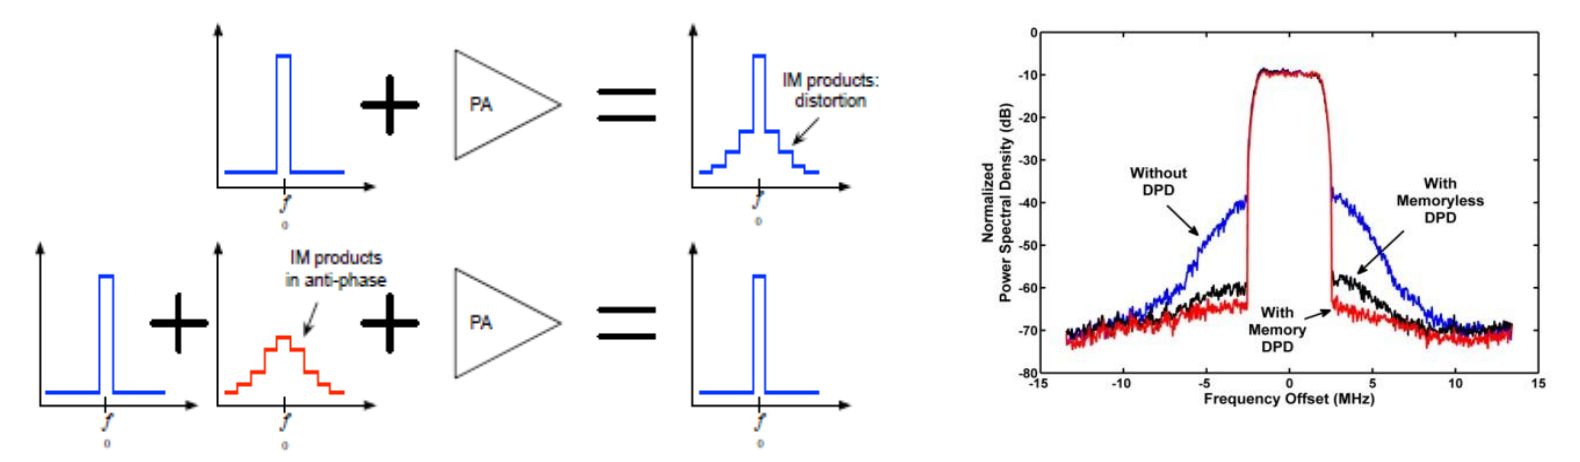
\includegraphics[width=0.5\linewidth]{DPD.png}
    \caption{DPD原理}
\end{figure}
\end{itemize}   
\end{frame}

	
\section{Technical Insight  }
\begin{frame}{Neural Network Architecture }
\begin{itemize}
    \item   RVTDCNN(实值延时卷积神经网络) \\
	~\\
	\begin{figure}[htpb]
		\begin{center}
			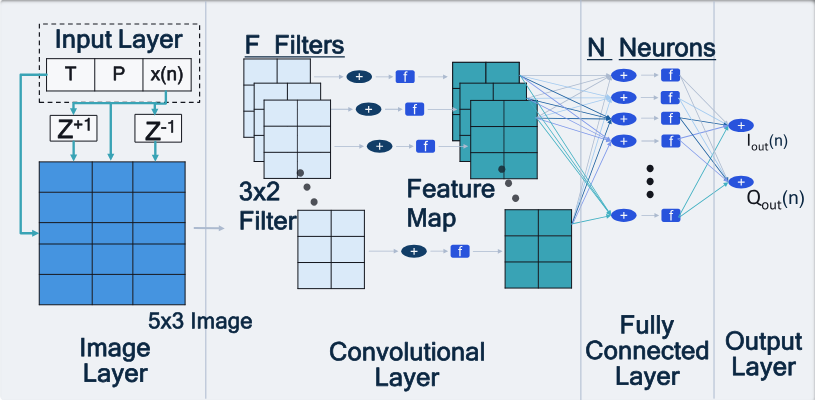
\includegraphics[width=0.5\linewidth]{RVTDCNN.png}
			\caption{RVTDCNN参考结构}
            \begin{itemize}
            \item 通过简单的卷积核滑动来覆盖历史序列 ，但感受野随层数L或卷积核大小K呈\textbf{线性增长} 。
            \end{itemize}
		\end{center}
	\end{figure}
\end{itemize}
\end{frame}

\begin{frame}{Neural Network Architecture }
\begin{itemize}
    \item   TCN (时间卷积网络) \\
\begin{figure}
    \centering
    \begin{minipage}{0.43\linewidth}
        \centering
        \includegraphics[width=\linewidth]{} 
\begin{figure}
            \centering
            \includegraphics[width=0.75\linewidth]{}
\begin{figure}
            \centering
            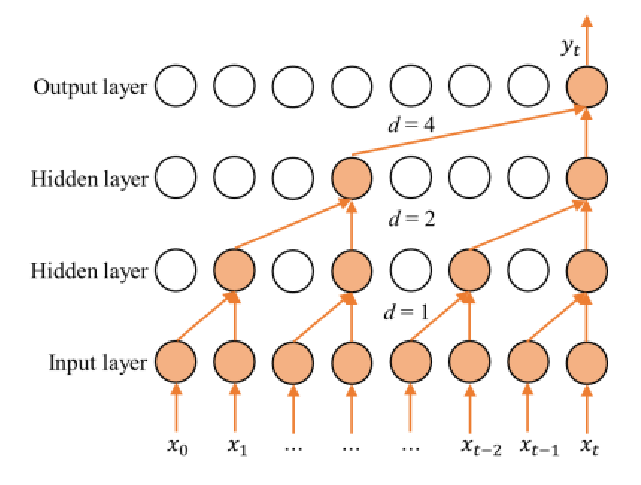
\includegraphics[width=0.75\linewidth]{TCN.png}
            \caption{TCN空洞机制}
        \end{figure}
                \end{figure}
    \end{minipage}
    \hfill
    \begin{minipage}{0.55\linewidth}
        \centering
        \includegraphics[width=\linewidth]{} 
\begin{itemize}
            \item 通过空洞卷积机制使得网络能够在不增加乘法器消耗的情况下，让感受野呈\textbf{指数级增长}。
~\\
 ~\\
 ~\\
            \item  残差连接允许网络在保持极低宽度的同时加深层数，解决了深层网络梯度消失的问题。
\end{itemize}
    \end{minipage}
\end{figure}
\end{itemize}
\end{frame}


       
\begin{frame}{Neural Network Architecture }
\begin{itemize}
    \item   LSTM(长短期记忆网络)\\
\begin{figure}
    \centering
    \begin{minipage}{0.43\linewidth}
        \centering
        \includegraphics[width=\linewidth]{} 
\begin{figure}
            \centering
            \includegraphics[width=0.75\linewidth]{}
\begin{figure}
            \centering
            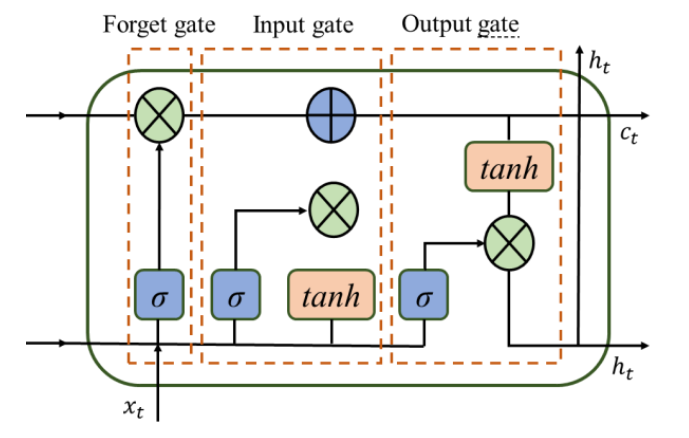
\includegraphics[width=0.75\linewidth]{LSTM.png}
            \caption{LSTM结构}
        \end{figure}
                \end{figure}
    \end{minipage}
    \hfill
    \begin{minipage}{0.55\linewidth}
        \centering
        \includegraphics[width=\linewidth]{} 
\begin{itemize}
            \item 引入了三个门控(输入门、遗忘门、输出门)，通过IIR特性来控制信息流，捕获极长序列中的历史依赖。
~\\
 ~\\
            \item 能够完美捕获功放深层的长程热效应与电荷陷阱记忆，处理高阶特征。
 ~\\
  ~\\
           \item 将宽带高频信号强行压缩进低维隐藏状态中，会产生严重的非线性信息丢失。
\end{itemize}
    \end{minipage}
\end{figure}
\end{itemize}
\end{frame}


\begin{frame}{Neural Network Architecture }
\begin{itemize}
    \item   DeltaGRU(时间稀疏差分GRU)\\
     ~\\
\begin{figure}
    \centering
    \begin{minipage}{0.4\linewidth}
        \centering
        \includegraphics[width=\linewidth]{} 
\begin{figure}
            \centering
            \includegraphics[width=0.75\linewidth]{}
\begin{figure}
            \centering
            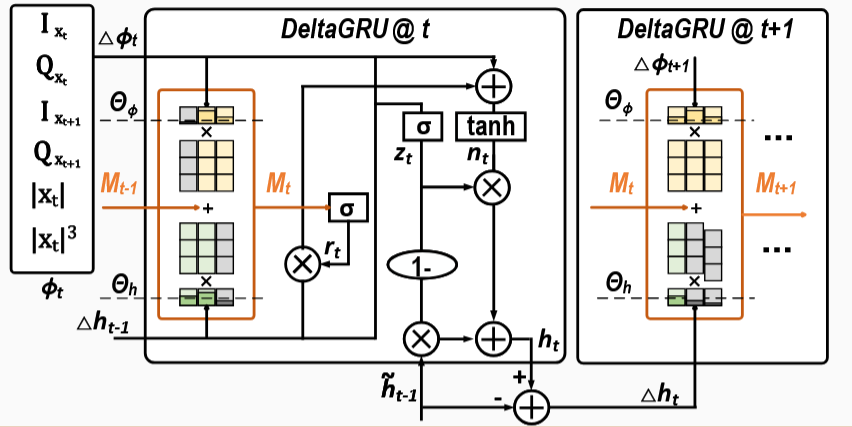
\includegraphics[width=1\linewidth]{DeltaGRU.png}
            \caption{DeltaGRU结构}
        \end{figure}
                \end{figure}
    \end{minipage}
    \hfill
    \begin{minipage}{0.58\linewidth}
        \centering
        \includegraphics[width=\linewidth]{} 
\begin{itemize}

\item DeltaGRU的更新公式如下：
     ~\\
    \begin{equation}
\mathbf{r}_t &= \sigma\left(\mathbf{M}_{r,t}\right) 
   \end{equation}
     \begin{equation}
\mathbf{z}_t &= \sigma\left(\mathbf{M}_{z,t}\right) 
   \end{equation}
     \begin{equation}
\mathbf{n}_t &= \tanh\left(\mathbf{M}_{n\phi,t} + \mathbf{r}_t \odot \mathbf{M}_{nh,t}\right) 
  \end{equation}
    \begin{equation}
\mathbf{h}_t &= \left(1 - \mathbf{z}_t\right) \odot \mathbf{h}_{t-1} + \mathbf{z}_t \odot \mathbf{n}_t
    \end{equation}
\end{itemize}
    \end{minipage}
\end{figure}
\end{itemize}
\end{frame}




\begin{frame}{Neural Network Architecture }
\begin{itemize}
    \item   DeltaGRU在常规 GRU 的基础上引入了差分阈值门控，只有当变化率超过设定的阈值时才会更新隐藏状态。 \\
	~\\
    	~\\
    \item 利用时序信号的稀疏性，跳过平缓波形处的计算,压低硬件的平均活跃实数乘法器。\\
~\\
	~\\
    \item 5G-A 宽带信号具有极高的采样率和 PAPR(峰均比)，稀疏性难以降低。

\end{itemize}
\end{frame}



\begin{frame}{Neural Network Architecture }
\begin{itemize}
    \item   BO-JANET(块正交JANET网络)\\
\begin{figure}
    \centering
    \begin{minipage}{0.43\linewidth}
        \centering
        \includegraphics[width=\linewidth]{} 
\begin{figure}
            \centering
            \includegraphics[width=0.75\linewidth]{}
\begin{figure}
            \centering
            \includegraphics[width=0.75\linewidth]{}
\begin{figure}
                \centering
                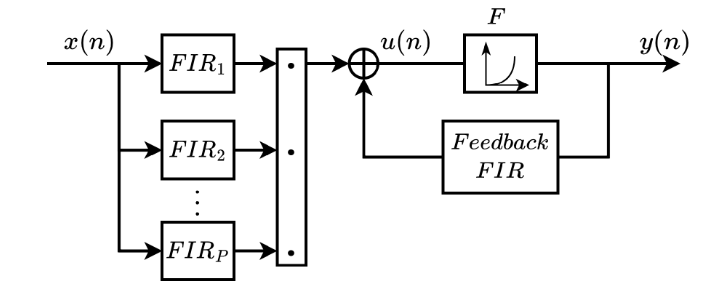
\includegraphics[width=1\linewidth]{BO-JANET.png}
            \end{figure}
                        \caption{BO-JANET的特征解耦}
        \end{figure}
                \end{figure}
    \end{minipage}
    \hfill
    \begin{minipage}{0.55\linewidth}
        \centering
        \includegraphics[width=\linewidth]{} 
\begin{itemize}
            \item 宽带高频信号的不同延迟项和交叉项之间存在极强的相关性。通过这组正交滤波器，提前将信号投影到正交基上，消除特征间的重叠干扰。
~\\
 ~\\
            \item 极大降低了后续神经网络的拟合难度，使得极小规模的网络也能高精度拟合。
 ~\\
  ~\\
           \item JANET 是 LSTM 的精简版(仅保留遗忘门)，用于捕获深层记忆。
\end{itemize}
    \end{minipage}
\end{figure}
\end{itemize}
\end{frame}
	

    
\section{Problem-Solving Strategy}
\begin{frame}{Problem-Solving Strategy}
\begin{itemize}
    \item  赛题核心矛盾：200MHz 宽带信号的强记忆效应要求极大的感受野，但 <800 等效实数乘法器使得常规网络(如 RVTDCNN)通过加深层数或增大卷积核来扩展感受野的思路难以解决。 \\
    ~\\
    \item 对于数据预处理，前期为了配合RNN变体神经网络的高算力开销，使用GMP作为神经网络的输入特征工程，通过分析数据集的特点，人工构造高阶记忆交叉项。\\
~\\
    \item 使用 RMS 归一化对齐数据，并计算 PA 物理反向增益 G，训练集采用步长(SL=32)进行高重叠切片，使网络学习平移不变性。\\
    ~\\
    \item 提出面向5G-A Pro宽带低复杂度的轻量级AI DPD算法架构——\textbf{EA-TCN (Envelope-Attention TCN/包络注意力时间卷积网络)}。
    ~\\

    \end{itemize}
\end{frame}


    \begin{frame}{Envelope-Attention TCN}
    \begin{itemize}
    \item 在网络结构上，我们显式定义了一阶线性增益与三阶无记忆物理旁路，处理静态的 AM-AM/AM-PM 畸变。\\
    ~\\
    \item 主干网络采用通道数 H=10、卷积核 K=5 的 4 层 TCN 网络，相比RVTDCNN极大的增加了感受野，处理高频率的热效应延迟。 \\
~\\
    \item 射频记忆效应的激化几乎完全由信号的“幅度包络”驱动，我们通过极轻量的门控网络生成注意力权重，聚焦于处理高功率突变点。\\
    ~\\
    \item EA-TCN 的等效实数乘法器为 778 个。

     \end{itemize}
    \end{frame}


    \begin{frame}{Envelope-Attention TCN}
    \begin{itemize}
    \begin{figure}[htb]
	\centering
	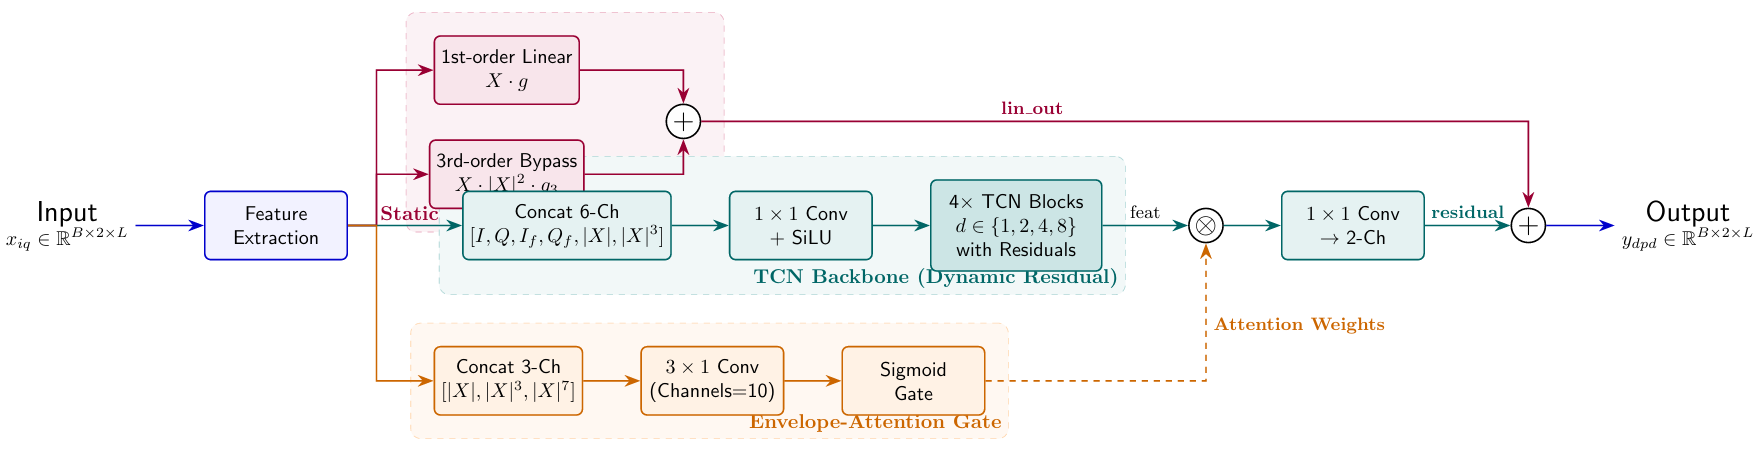
\includegraphics[width=\linewidth]{pic/EA-TCn.png}
    \caption{EA-TCN结构}
\end{figure}
    \item 等效实数乘法器：2 * 4 + 6 * 10 + (10 * 10 + 5 * 10) * 4 + 2 * 10 + 10 * 3 * 3 = 778
     \end{itemize}
    \end{frame}


	
\section{Simulation}
\begin{frame}{Simulation}
\begin{itemize}
    \item 为了评估拟合程度，使用NMSE评估神经网络拟合误差，赛题要求等价为NMSE = -40dB。\\
    ~\\
\begin{figure}
        \centering
        \includegraphics[width=0.5\linewidth]{}
            \centering
            \includegraphics[width=0.5\linewidth]{}
\begin{figure}
            \centering
            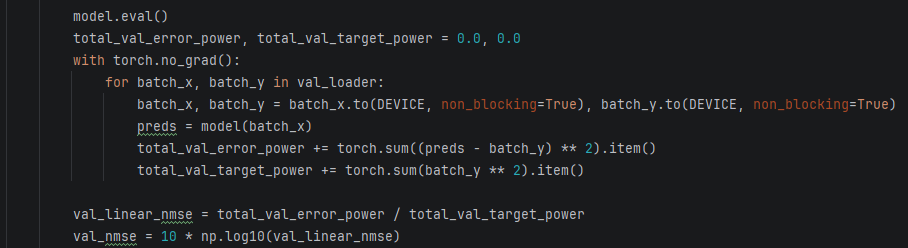
\includegraphics[width=0.75\linewidth]{NMSE.png}
            \caption{NMSE计算代码}
        \end{figure}
        \begin{itemize}
    \item 累计整个验证集的全局误差功率，除以全局目标功率，最后统一取对数。 
        \end{itemize}
    \end{figure}
\end{itemize}
\end{frame}


\begin{frame}{Simulation}
\begin{itemize}
    \item 设置滑动窗口SL = 32，验证集测试时关闭滑动窗口重叠，模拟基站 FPGA 在真实业务中的连续流式处理状态。\\
    ~\\
    \item 解题策略1：限制800乘法器。在 MACs = 778个的 EA-TCN 架构下：
\begin{figure}
      \centering
      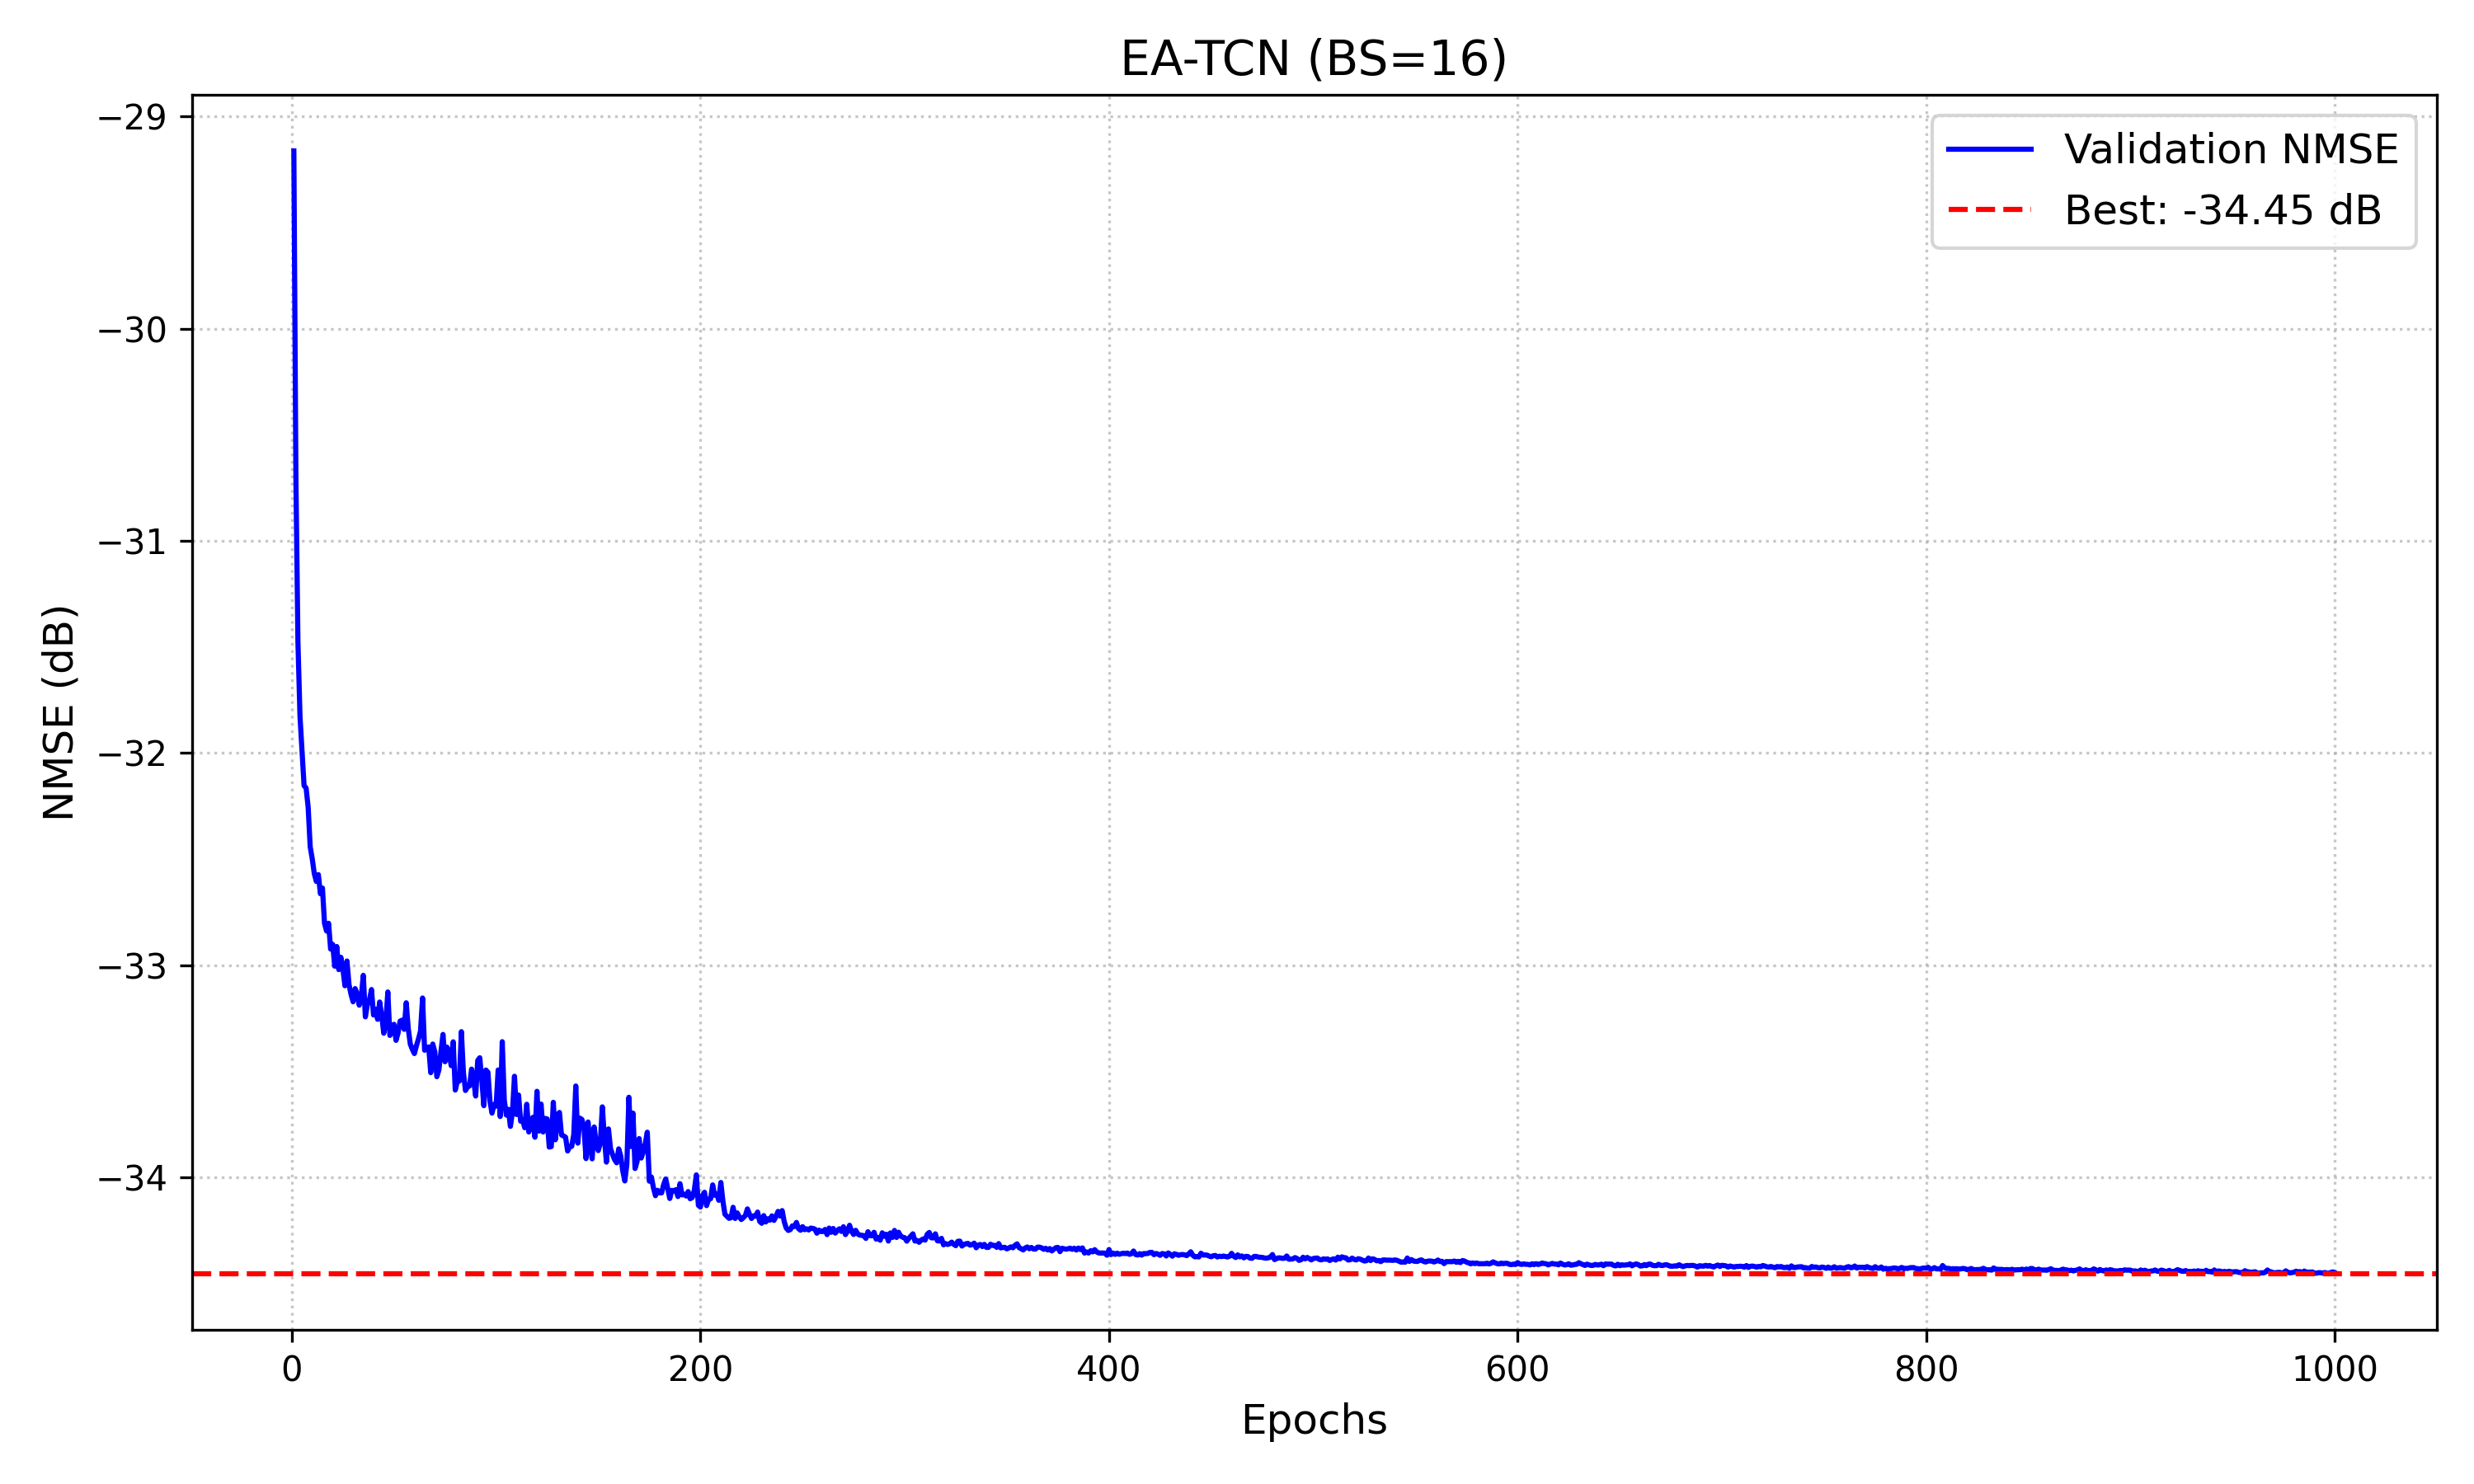
\includegraphics[width=0.5\linewidth]{111111111.png}
      \caption{当前架构的NMSE}
  \end{figure}
\end{itemize}
\end{frame}



\begin{frame}{Simulation}
\begin{itemize}
    \item   当在我们的 EA-TCN 的架构下，增加通道数或者加深神经网络层数：\\
    ~\\
\begin{figure}
    \centering
    \begin{minipage}{0.48\linewidth}
        \centering
        \includegraphics[width=\linewidth]{} 
\begin{figure}
            \centering
            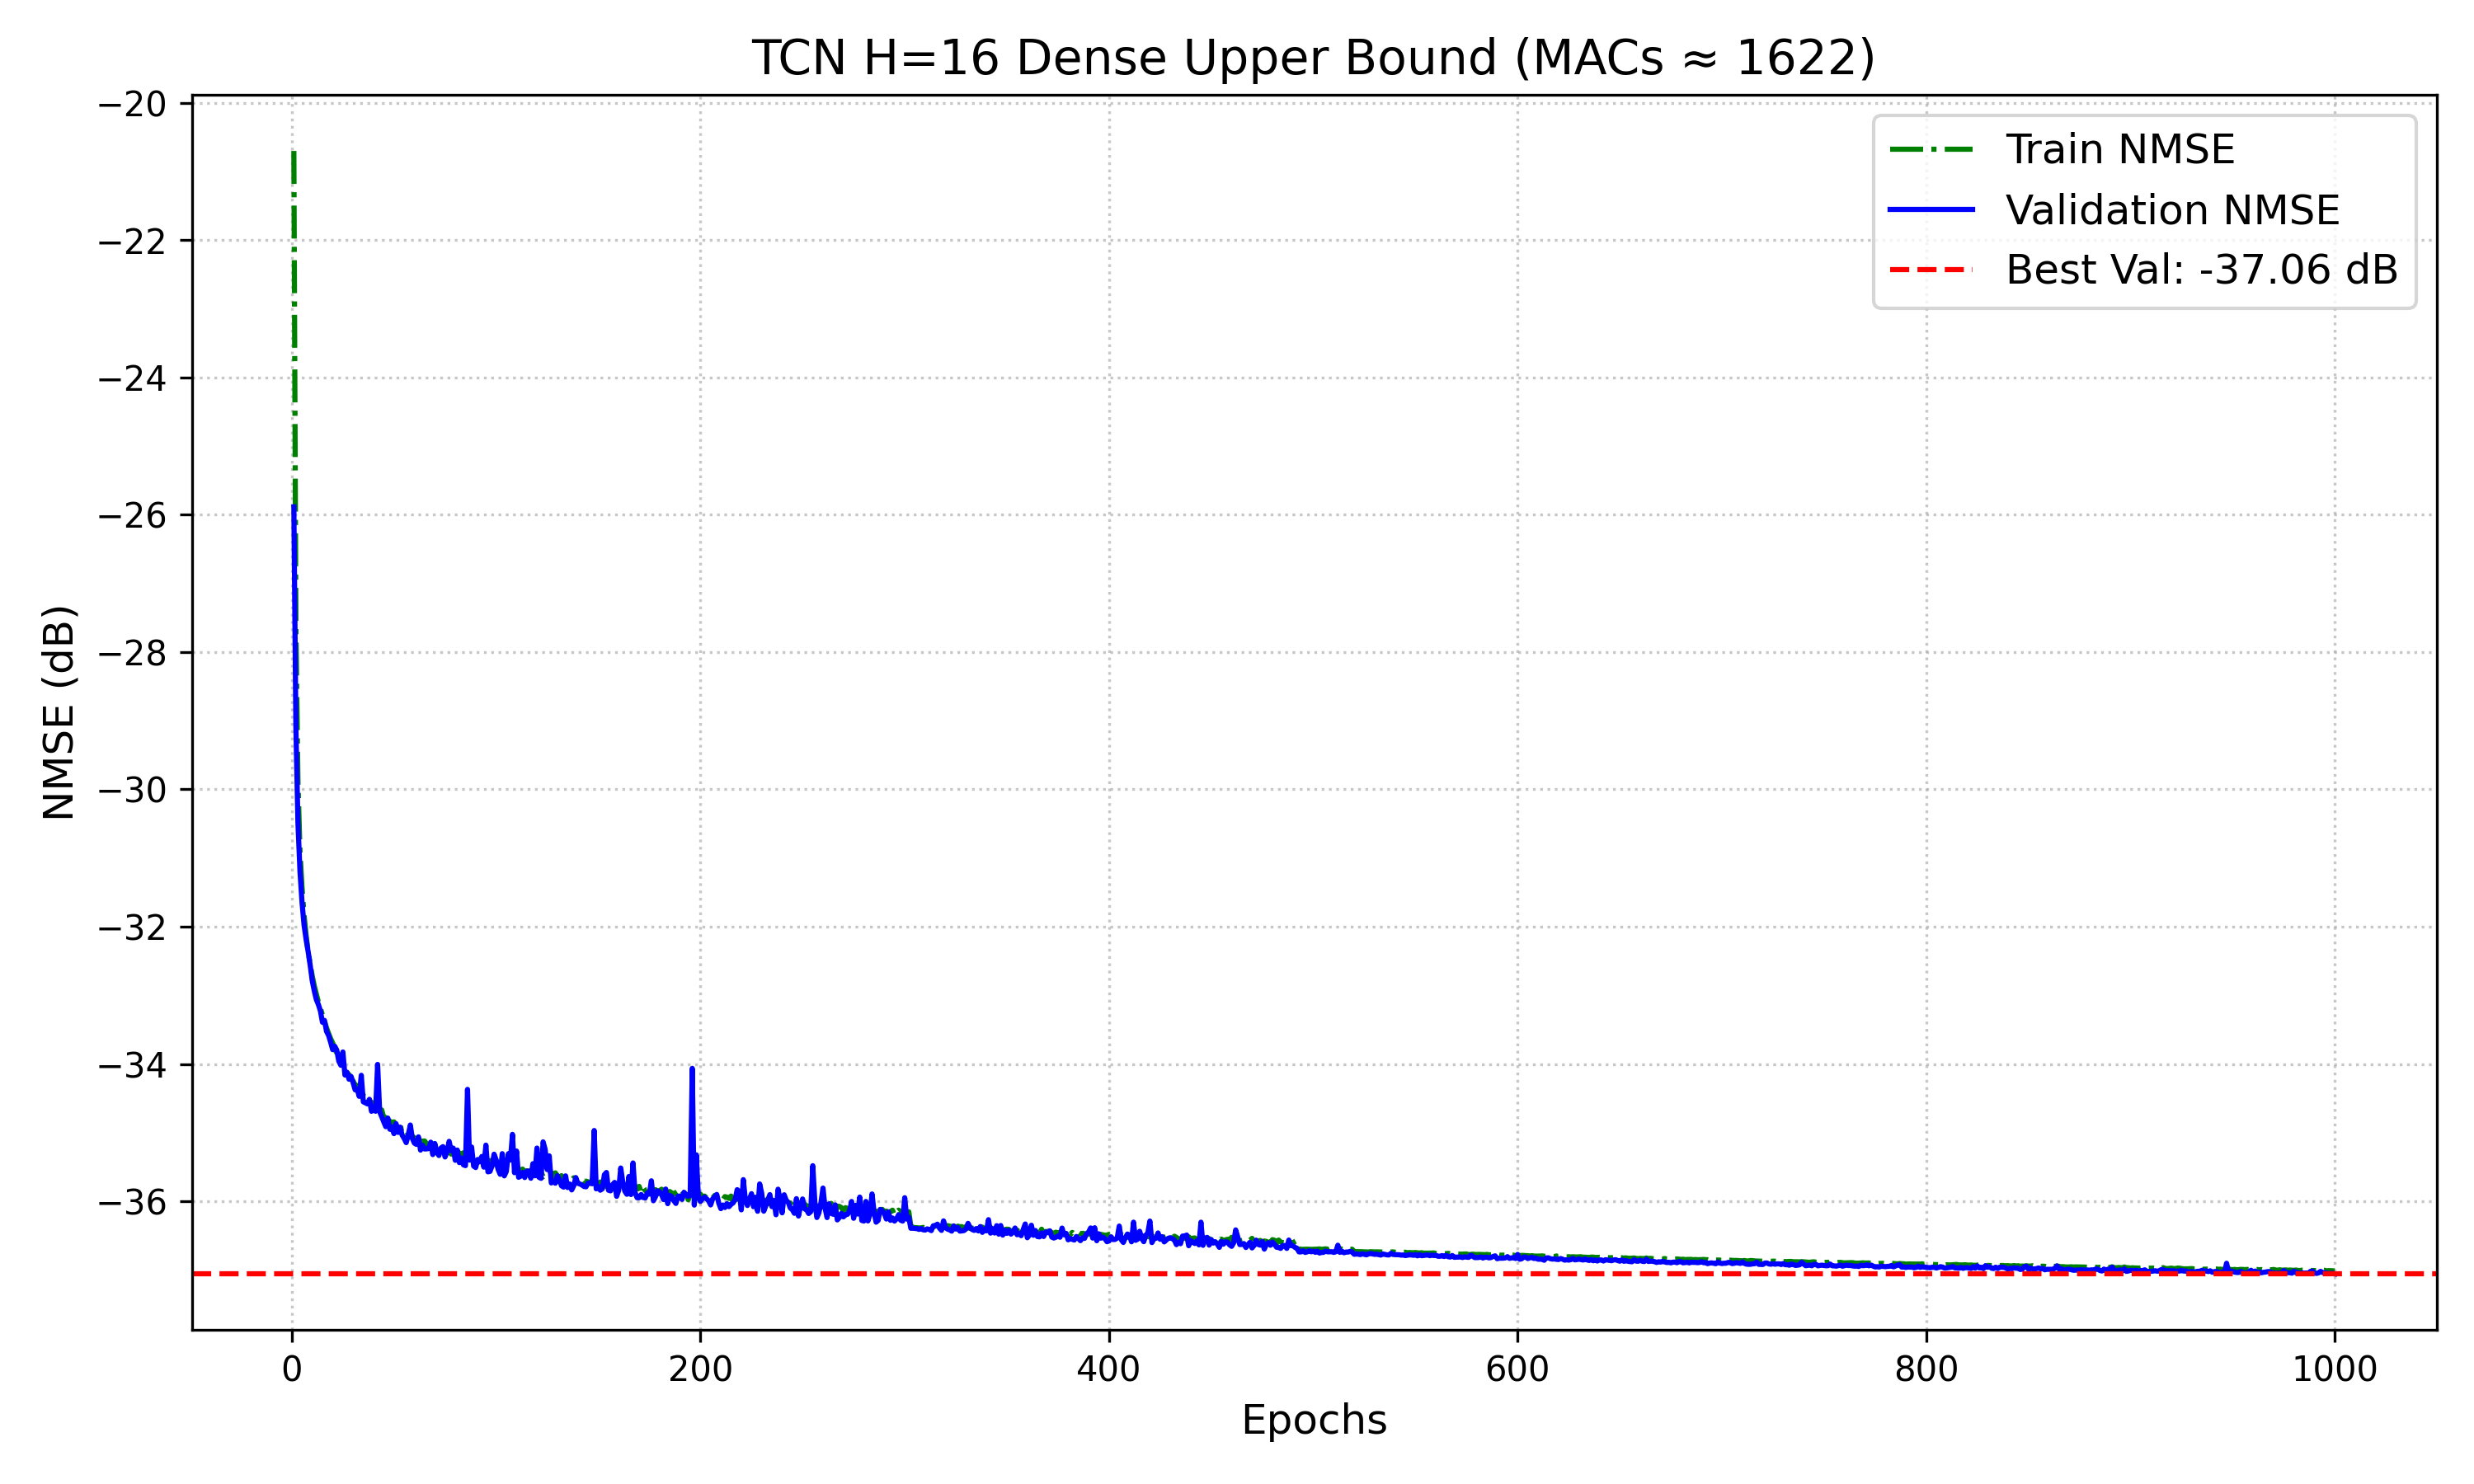
\includegraphics[width=0.75\linewidth]{EA-TCN16.png}
        \end{figure}
                \caption{H=16的EA-TCN的NMSE}
    \end{minipage}
    \hfill
    \begin{minipage}{0.48\linewidth}
        \centering
        \includegraphics[width=\linewidth]{} 
\begin{figure}
            \centering
            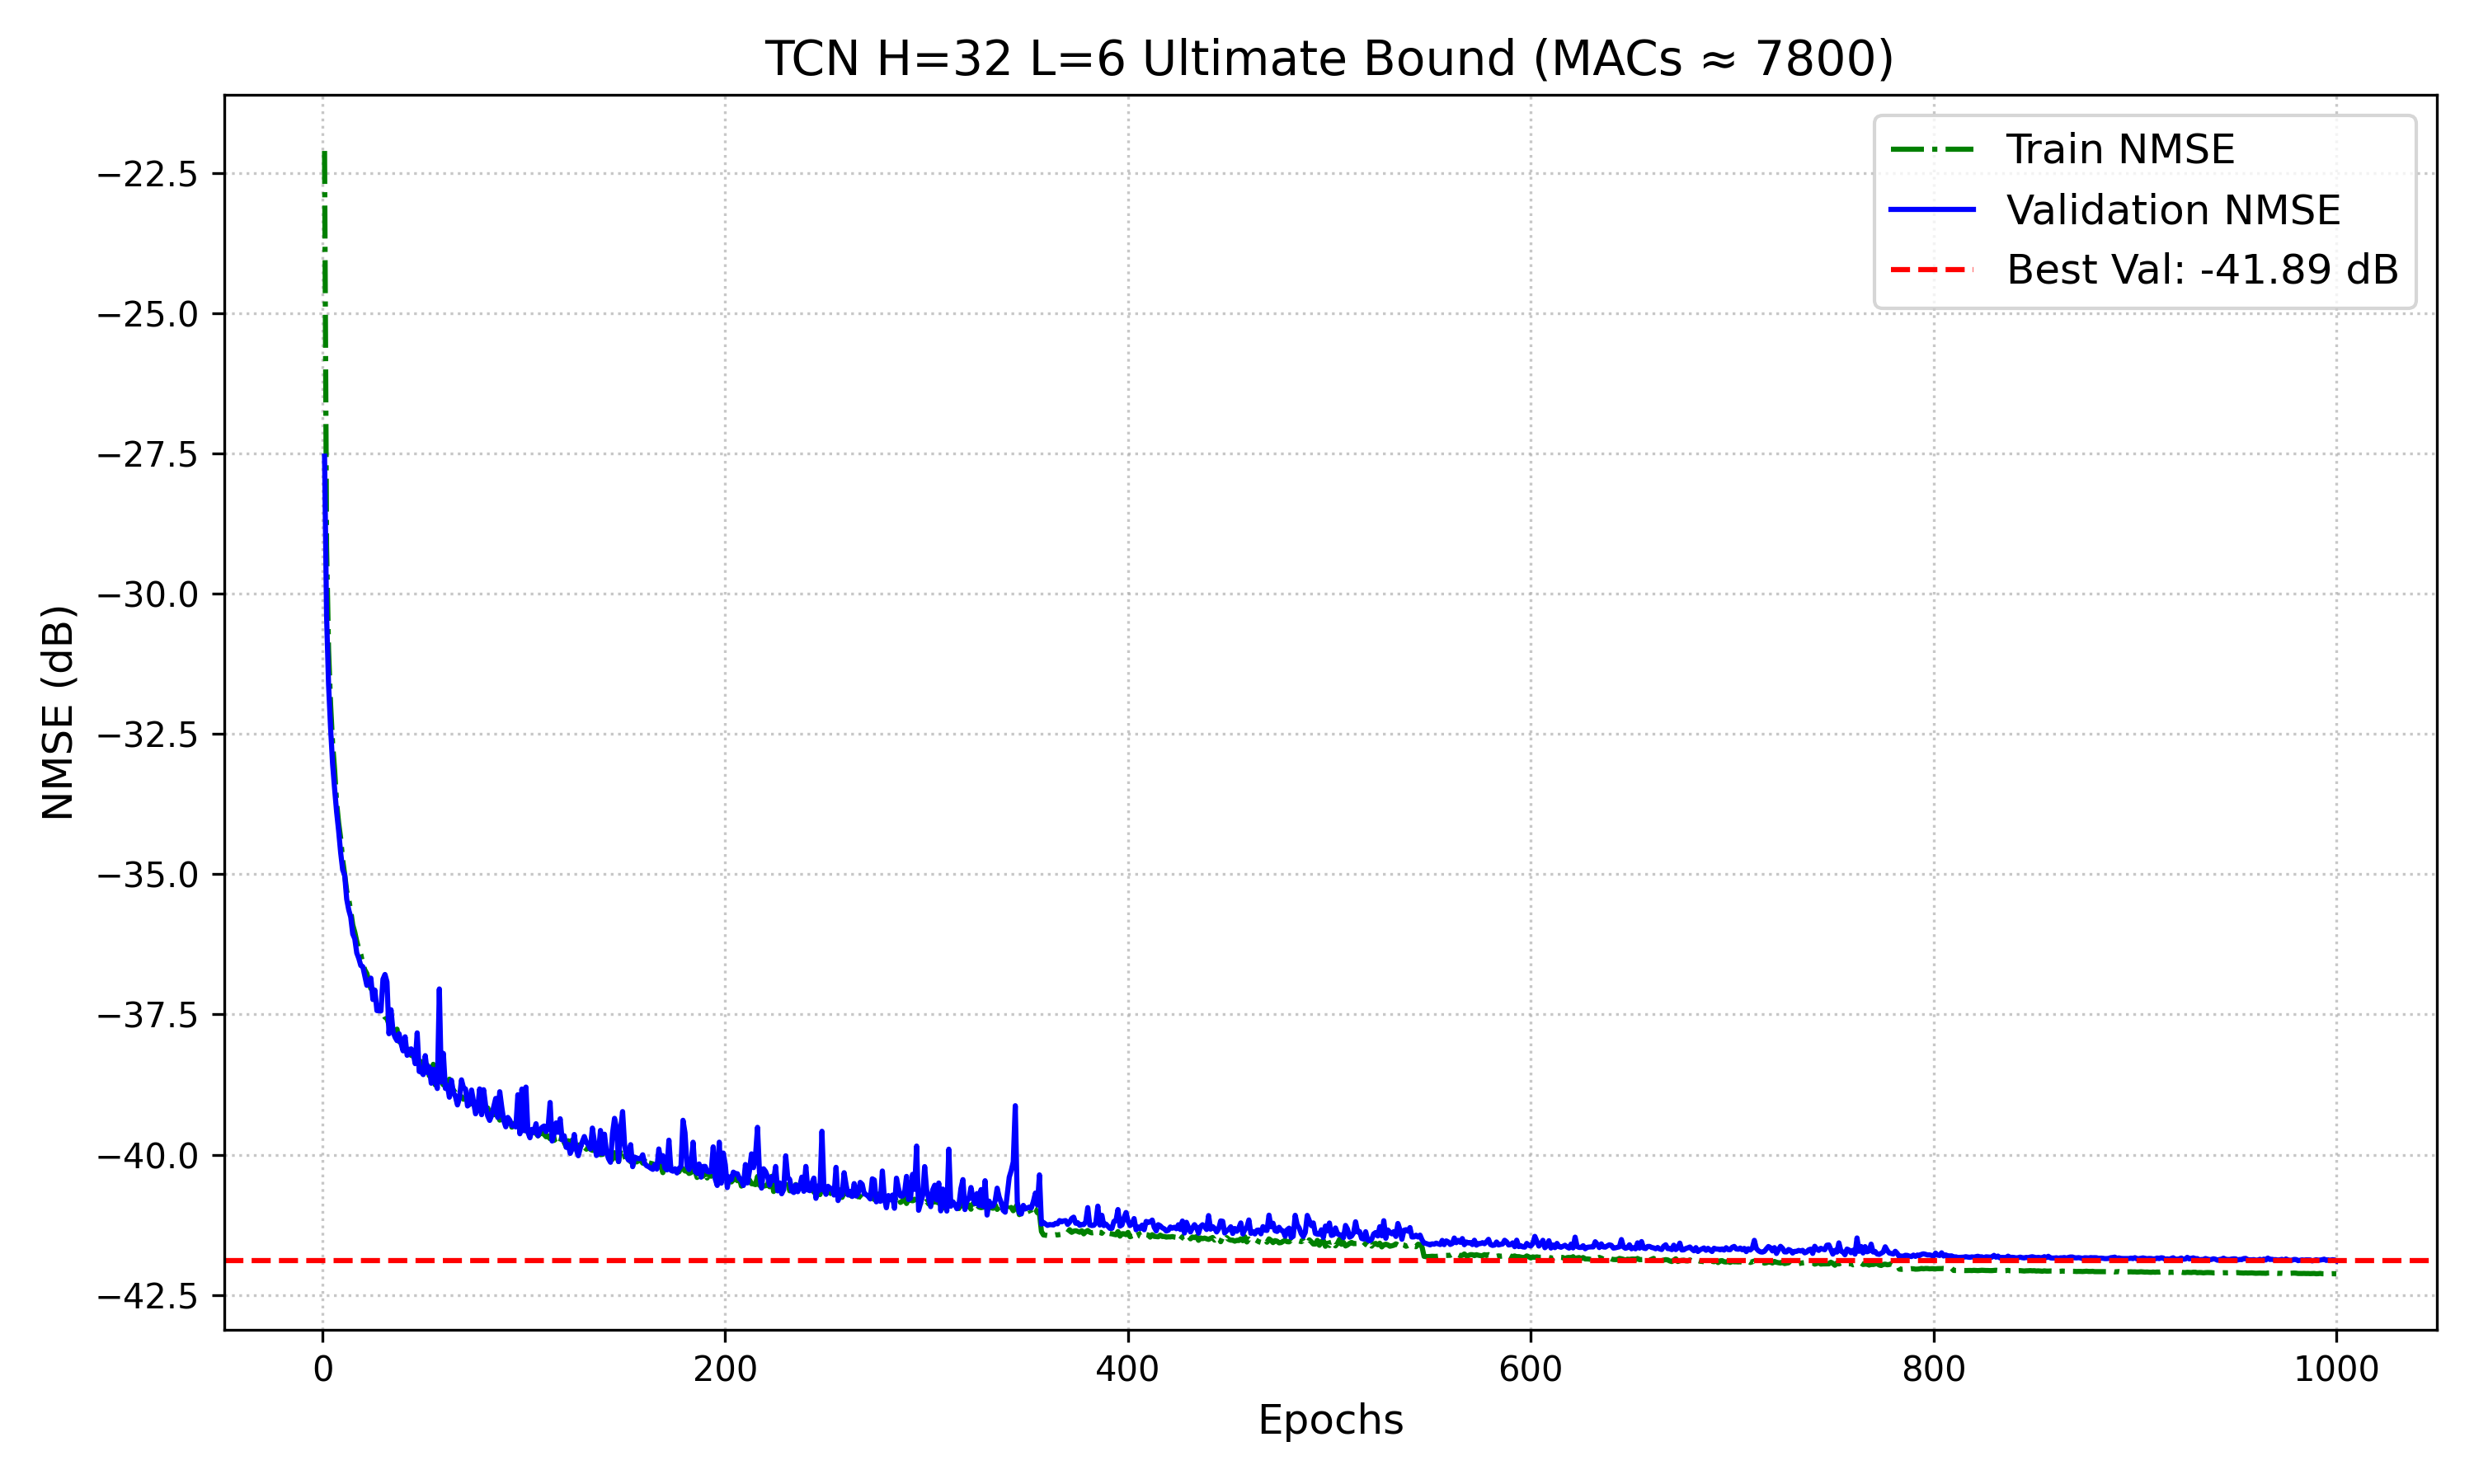
\includegraphics[width=0.75\linewidth]{-41.89dB.png}
        \end{figure}
                \caption{H=32的EA-TCN的NMSE}
    \end{minipage}
    \begin{itemize}
    \\
    ~\\
    \item  将网络隐藏层扩展（H=32），精度升至 -41.89 dB，证明该架构具有极强的非线性提取潜力。 
    \end{itemize}
\end{figure}
\end{itemize}
\end{frame}


\begin{frame}{Simulation}
\begin{itemize}
    \item 当前思路为限制乘法器在800以内，改进注意力机制，微调超参数。同时，也探讨改进架构或者学习方式。\\
    \item 尝试通过直接学习架构 (DLA) 级联EA-TCN，引入高精度的PA作为教师，引导EA-TCN进行端到端联合训练。
\begin{figure}
  \begin{figure}
      \centering
      \includegraphics[width=0.8\linewidth]{}
\begin{figure}
          \centering
          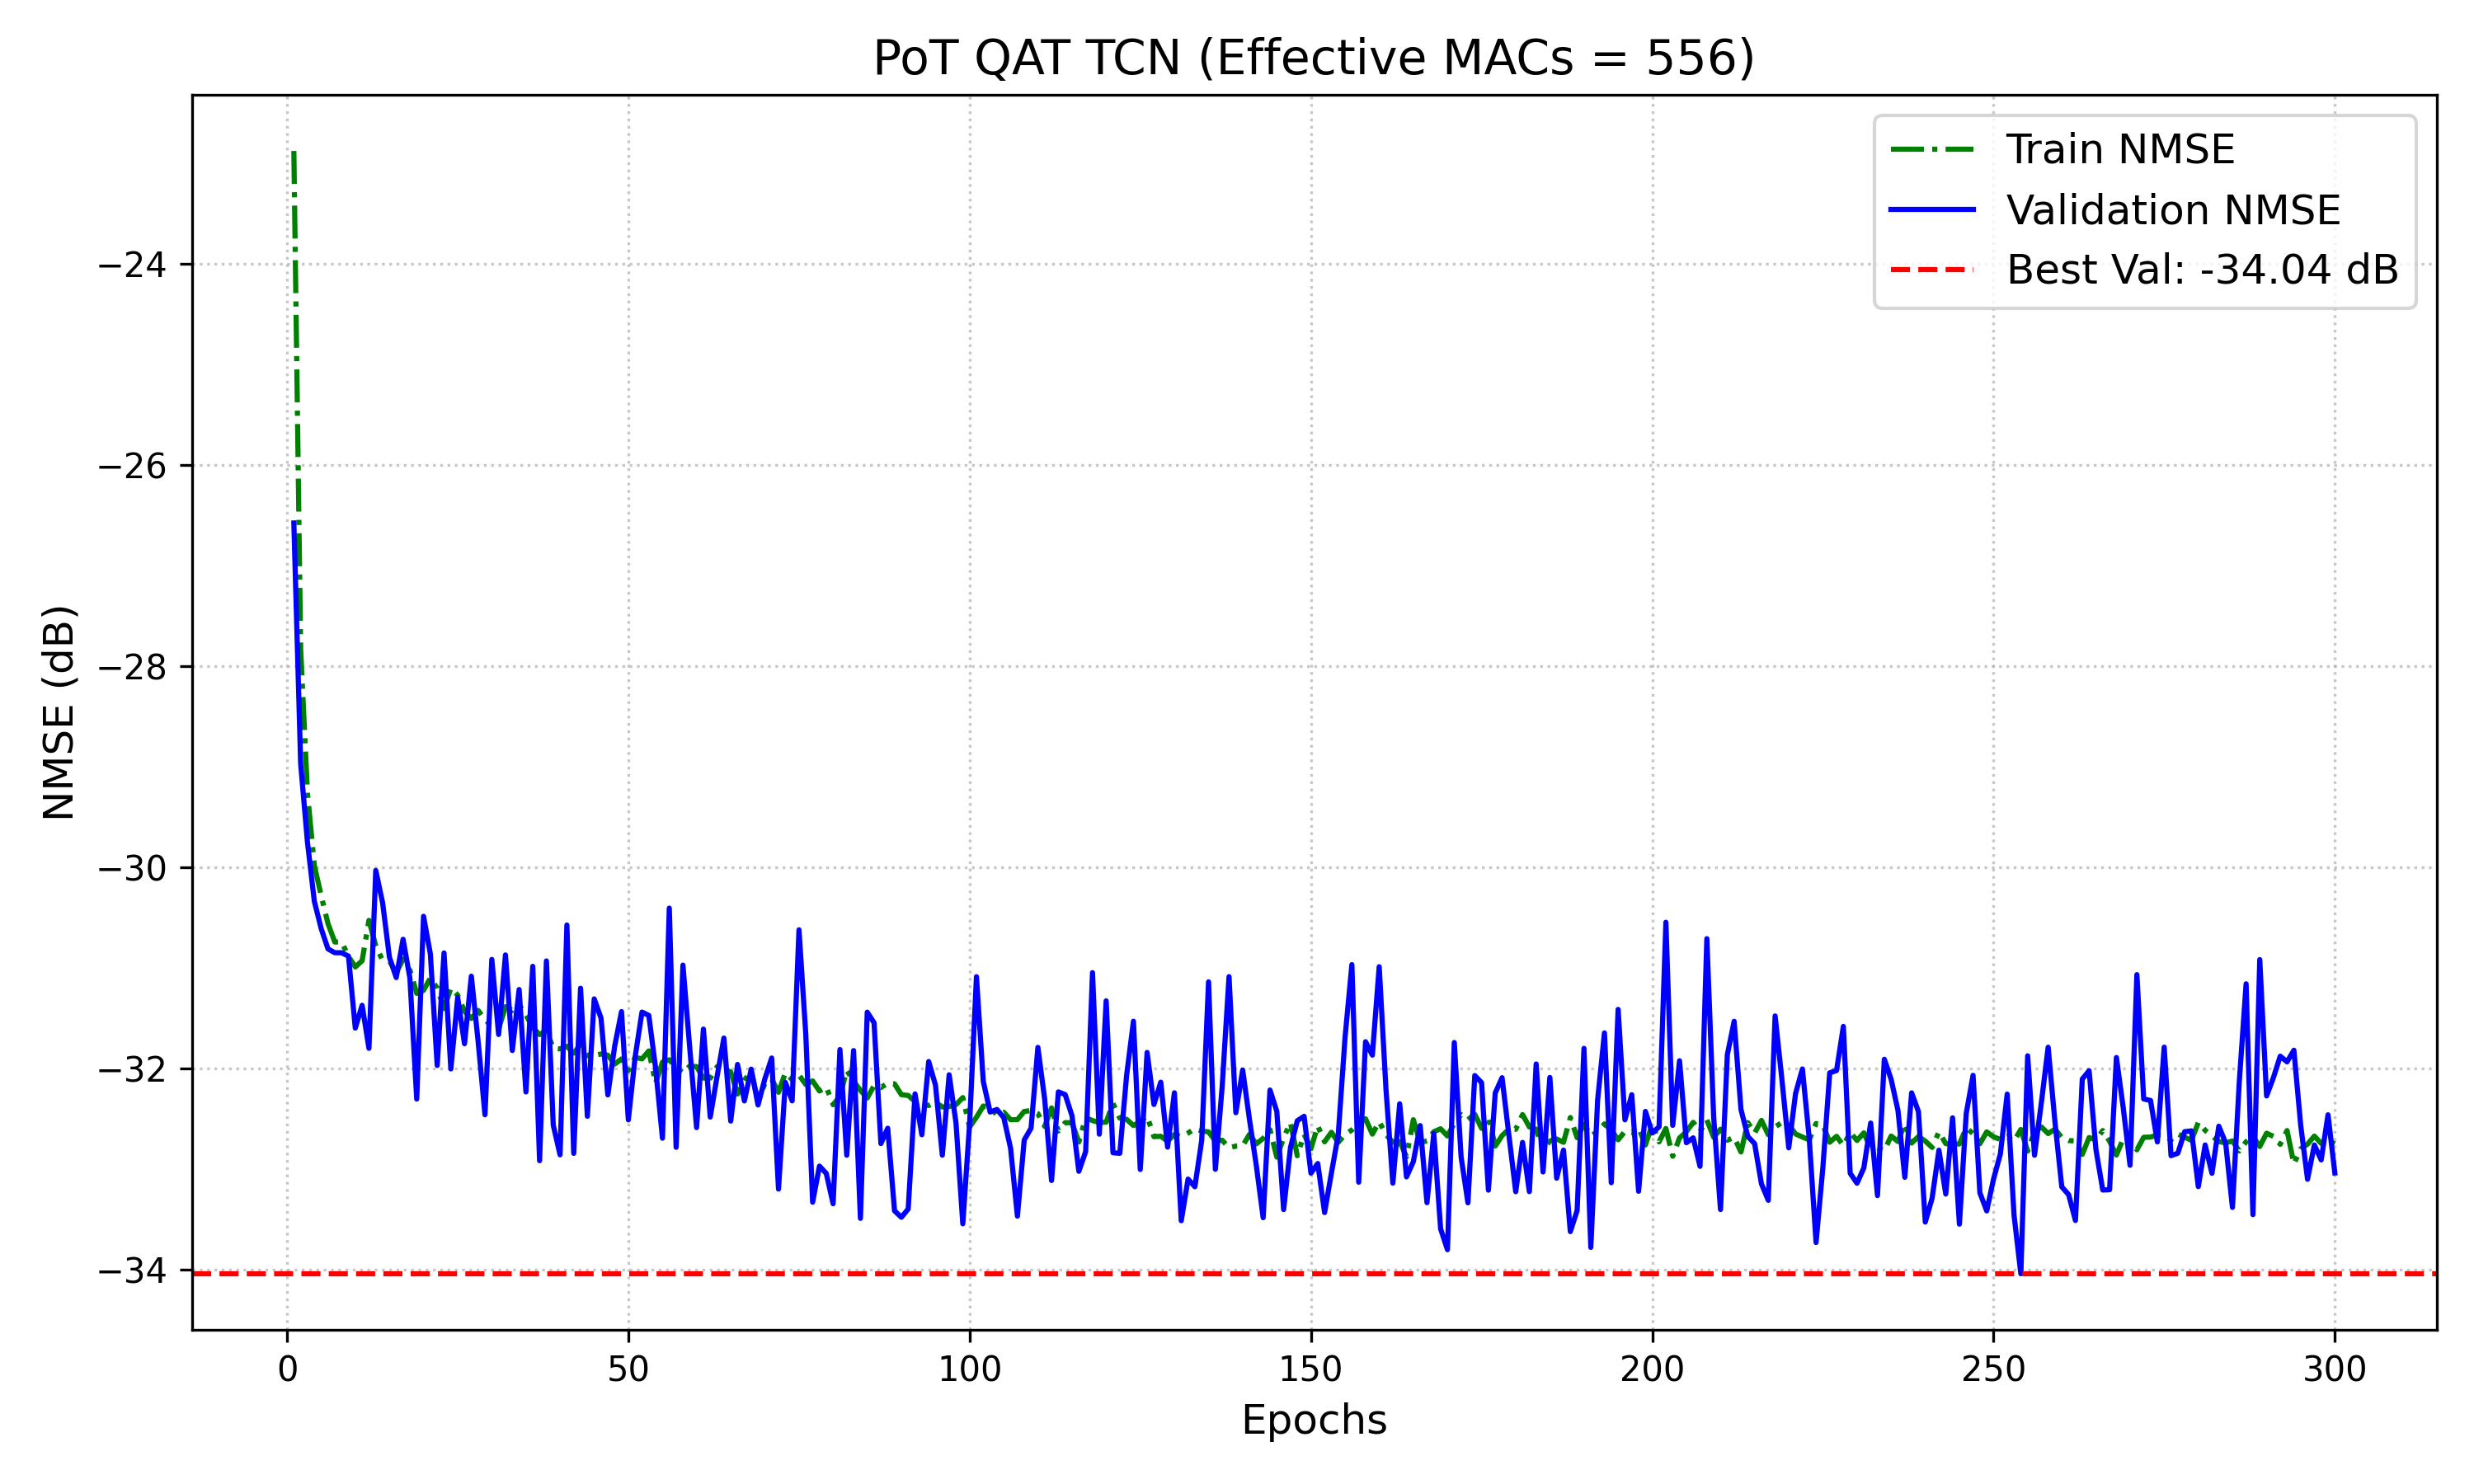
\includegraphics[width=0.5\linewidth]{DLA.png}
      \end{figure}
            \caption{目前DLA下的NMSE}
  \end{figure}
\end{figure}
\end{itemize}
\end{frame}



\section{Conclusion}
\begin{frame}{Conclusion}
\begin{itemize}
    \item 当前工作总结：在严苛的算力受限场景下，物理先验架构比数学优化(DLA/RNN/量化)更有效，收敛更快。(EA-TCN在5060ti的cuda核心加速下，每轮约1s，5min基本达到收敛,相反RNN方法计算H耗费大量时间)。\\
    ~\\
     ~\\
    \item 未来工作方向：先用层数更深的TCN网络达到拟合精度，再进行稀疏化训练和网络剪枝/训练精度更高的神经网络作为教师PA，继续探索DLA级联方式，加入量化感知以便轻量化部署硬件。\\
    ~\\
     ~\\
    \item 结题其他流程：将训练好的模型封装，验证赛题ACLR指标，总结解题全流程，完成结题任务书。\\
    ~\\
\end{itemize}
\end{frame}


\section{References}
\begin{frame}[allowframebreaks]
    \bibliography{ref}
    \bibliographystyle{alpha}
    % If too many references, use this command to resize：
    % \tiny\bibliographystyle{alpha}
   \\% 参考文献列表
\begin{thebibliography}{99}
\bibitem{1} Q. Zhang, C. Jiang, G. Yang, R. Han, and F. Liu, ``Block-Oriented Recurrent Neural Network for Digital Predistortion of RF Power Amplifiers,'' \emph{IEEE Transactions on Microwave Theory and Techniques}, vol. 72, no. 7, pp. 3875--3885, Jul. 2024, doi: 10.1109/TMTT.2023.3337939.

\bibitem{2} J. D. Domingues, A. Prata, and J. Stulemeijer, ``Improved Temperature- and Power-Dependent Convolutional NN-Based PA,'' \emph{IEEE Microwave and Wireless Technology Letters}, vol. 33, no. 6, pp. 879--882, Jun. 2023, doi: 10.1109/LMWT.2023.3268796.

\bibitem{3} K. Zuo, ``Integrated Forecasting Models Based on LSTM and TCN for Short-Term Electricity Load Forecasting,'' in 2023 9th International Conference on Electrical Engineering, Control and Robotics (EECR), Feb. 2023, pp. 207--211, doi: 10.1109/EECR56827.2023.10149951.

\bibitem{4} X. Hu et al., ``Convolutional Neural Network for Behavioral Modeling and Predistortion of Wideband Power Amplifiers,'' \emph{IEEE Transactions on Neural Networks and Learning Systems}, vol. 33, no. 8, pp. 3923--3937, Aug. 2022, doi: 10.1109/TNNLS.2021.3054867.

\bibitem{5} Y. Wu et al., ``MP-DPD: Low-Complexity Mixed-Precision Neural Networks for Energy-Efficient Digital Predistortion of Wideband Power Amplifiers,'' \emph{IEEE Microw. Wireless Tech. Lett.}, vol. 34, no. 6, pp. 817--820, Jun. 2024, doi: 10.1109/LMWT.2024.3386330.

\bibitem{6} Y. Wu, A. Li, and C. Gao, ``OpenDPDv2: A Unified Learning and Optimization Framework for Neural Network Digital Predistortion,'' arXiv:2507.06849, Dec. 2025, doi: 10.48550/arXiv.2507.06849.

\bibitem{7} G. Somasundaram, J. C. Mayeda, D. Y. C. Lie, and J. Lopez, ``Effective Linearization of Millimeter-Wave Power Amplifiers Using LUT-Based Digital Predistortion (DPD),'' in 2022 IEEE Texas Symposium on Wireless and Microwave Circuits and Systems (WMCS), Waco, TX, USA: IEEE, Apr. 2022, pp. 1--4, doi: 10.1109/WMCS55582.2022.9866349.

\bibitem{8} Q. Xie, Y. Wang, J. Ding, Z. Guo, and J. Niu, ``Low Complexity Convolutional Neural Network Digital Predistortion for Radio Frequency Power Amplifiers,'' in 2024 IEEE 24th International Conference on Communication Technology (ICCT), Chengdu, China: IEEE, Oct. 2024, pp. 1639--1643, doi: 10.1109/ICCT62411.2024.10946304.

\bibitem{9} W. Wang, T. Wu, J. Duan, Y. Tan, and P. Yu, ``Lightweight Complex-Valued Delay RBFNN for Predistortion of Wideband Power Amplifiers,'' in 2025 13th International Conference on Intelligent Computing and Wireless Optical Communications (ICWOC), Jun. 2025, pp. 327--333, doi: 10.1109/ICWOC65853.2025.11151110.

\bibitem{10} G. Zhao, K. Ying, Q. Wen, J. Zhang, and L. Gui, ``Transfer Learning with Transformer and LSTM for Digital Pre-distortion of Terahertz/mmWave Transceiver,'' in ICASSP 2025 - 2025 IEEE International Conference on Acoustics, Speech and Signal Processing (ICASSP), Apr. 2025, pp. 1--5, doi: 10.1109/ICASSP49660.2025.10890748.
\end{thebibliography}
\end{frame}

\end{document}